\documentclass[10pt]{article}
\usepackage{icmlko}

\icmlmeta{IP 파운데이션 월드모델}{62}{네 번 짚었고 네 번 틀렸다}{주성분이 오토인코더를 이기는 이유를 넷으로 좁혀 전부 검정했는데 전부 기각됐다}

\begin{document}

\twocolumn[
\icmlheader

\begin{abstract}
노트 61이 신경망 격차의 61\%를 설명했다 --- 표현을 라벨로 학습한 것. 라벨을
빼고 오토인코더로 바꾸니 $+$0.2004에서 $+$0.3078로 올랐다. 그런데 도메인별
주성분 분석($+$0.3506)에는 여전히 0.043 뒤진다. 그 나머지를 설명할 후보를
넷으로 좁혀 전부 검정했다. \textbf{네 번 다 틀렸다.} (1) 비선형이 불리한가 ---
선형 오토인코더는 $+$0.2694로 \emph{더} 나쁘다. (2) 공유가 불리한가 --- 도메인마다
따로 학습한 오토인코더는 $+$0.2722로 \emph{더} 나쁘다. (3) 프로크루스테스가
직교 회전이니 잠재도 직교 좌표계여야 하는가 --- 백색화해도 $+$0.3083으로
변화가 없다. (4) 입력 열 절반이 마스크라 복원에 용량을 낭비하는가 --- 값 열만
복원해도 $+$0.3009로 오히려 조금 나쁘다. 자기지도 변형도 하나 더 시험했다 ---
축 하나를 가리고 맞히는 마스킹 복원은 $+$0.2405로 가장 나쁘다. \textbf{결과적으로
여러 변형 중 가장 단순한 것(공유 오토인코더 · 전체 재구성)이 최선이고, 그것도
닫힌 해에 0.043 못 미친다.} 원인을 모른다. 네 가지 그럴듯한 설명이 전부
틀렸다는 것만 안다.
\end{abstract}
]

\section{후보를 넷으로 좁혔다}

노트 61 이후 남은 격차는 0.043이다(도메인별 PCA $+$0.3506 대 공유 오토인코더
$+$0.3078). 설명할 만한 것이 넷 있었다.

\begin{figure}[t]
\centering
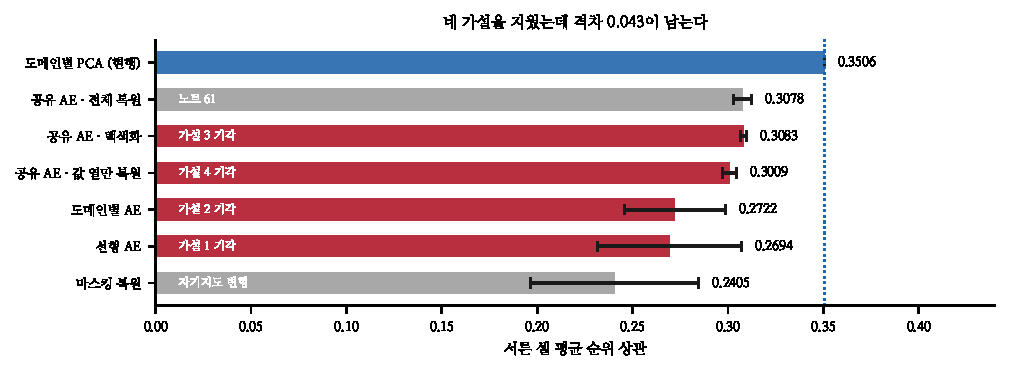
\includegraphics[width=\textwidth]{figs/fourwrong.pdf}
\caption{일곱 변형. 붉은 것이 기각된 가설이다.}
\end{figure}

\begin{table}[t]
\centering\tsize
\caption{변형별 서른 셀 평균 순위 상관. 씨앗 셋.}
\begin{tabular}{lrl}
\toprule
구성 & $\rho$ & 판정 \\
\midrule
도메인별 PCA(현행) & \textbf{$+$0.3506} & 기준 \\
공유 AE · 백색화 & $+$0.3083 & 가설 3 기각 \\
공유 AE · 전체 복원 & $+$0.3078 & 노트 61 \\
공유 AE · 값 열만 복원 & $+$0.3009 & 가설 4 기각 \\
도메인별 AE & $+$0.2722 & 가설 2 기각 \\
선형 AE & $+$0.2694 & 가설 1 기각 \\
마스킹 복원 & $+$0.2405 & 자기지도 변형 \\
\bottomrule
\end{tabular}
\end{table}

\paragraph{가설 1 --- 비선형이 불리하다}
PCA는 선형이고 오토인코더는 Tanh를 쓴다. 표본이 작으니 비선형이 과적합했을
수 있다. \textbf{선형 오토인코더가 $+$0.2694로 더 나쁘다.} 비선형이 오히려
유리하다.

\paragraph{가설 2 --- 공유가 불리하다}
PCA는 도메인마다 따로 계산되고 오토인코더는 하나를 공유한다. 도메인마다 축의
관계가 다르니 공유가 뭉갤 수 있다. \textbf{도메인별 오토인코더가 $+$0.2722로 더
나쁘다.} 도메인당 62--900건에서는 공유가 정규화 역할을 한다.

\paragraph{가설 3 --- 잠재가 직교하지 않다}
프로크루스테스는 직교 회전을 찾는다. 주성분은 서로 직교하고 분산 순으로
정렬돼 있는데 오토인코더 잠재는 아무 좌표계나 쓴다. \textbf{백색화해도
$+$0.3083으로 변화가 없다.}

\paragraph{가설 4 --- 마스크 복원에 용량을 쓴다}
입력 열 열 개 중 다섯이 마스크다. 오토인코더가 그것까지 복원하느라 용량의
절반을 쓴다. \textbf{값 열만 복원해도 $+$0.3009로 오히려 조금 나쁘다} ---
마스크 복원이 정규화 역할을 하고 있었다.

\claimx{주성분이 오토인코더를 0.043 앞서는 이유를 모른다. 비선형 · 공유 ·
직교성 · 복원 대상 넷을 검정해 전부 기각했다.}{남은 후보는 최적화다 --- PCA는
닫힌 해로 전역 최적이고 오토인코더는 경사하강으로 지역 최적에 머문다. 잠재
차원이 둘이라 지역 최적이 많지 않을 것 같지만 확인하지 않았다.}

\section{자기지도 변형도 최선이 가장 단순한 것이었다}

축 하나를 무작위로 가리고 맞히게 하는 마스킹 복원을 시험했다. 결측이 많은
이 자료에 맞는 목적함수이고 표 형식 사전학습에서 흔히 쓴다. \textbf{$+$0.2405로
가장 나쁘다.}

이유를 짐작하면 --- 축 하나를 다른 축으로 맞히는 것은 \emph{축 간 상관}을
학습하는 일이고, 그 상관이 도메인마다 다르다. 공유 인코더가 그것을 하나로
뭉개면 어느 도메인에서도 안 맞는 표현이 된다.

\begin{quote}\fontsize{9.5}{11.5}\selectfont
일곱 변형 중 가장 단순한 것 --- 공유 오토인코더에 전체 재구성 --- 이 최선이다.
그리고 그것도 닫힌 해에 못 미친다. 노트 60부터 세 노트에 걸쳐 신경망 쪽에서
얻은 것은 \textbf{설명}이지 성능이 아니다.
\end{quote}

\section{여기까지의 정리}

\begin{table}[t]
\centering\tsize
\caption{신경망과 선형의 격차 0.180.}
\begin{tabular}{lrr}
\toprule
원인 & 몫 & 상태 \\
\midrule
라벨로 표현을 학습(노트 61) & 0.110 & 설명됨 \\
정렬을 학습으로 대체(노트 60) & 0.030 & 설명됨 \\
\textbf{나머지} & \textbf{0.043} & \textbf{미상} \\
\bottomrule
\end{tabular}
\end{table}

76\%는 설명됐고 24\%는 남았다. 그리고 설명된 부분이 실무에 주는 지침은
분명하다 --- \textbf{다중 도메인 표현은 라벨로 빚지 말고, 정렬은 닫힌 해로
계산하라.} 현행 파이프라인이 이미 둘 다 하고 있다.

\section{한계}

\begin{itemize}[leftmargin=1.1em,itemsep=0.15em]
\item 최적화 가설을 검정하지 않았다. 여러 초기값에서 최선을 고르거나 학습률을
      훑으면 갈린다.
\item 각 변형을 씨앗 셋으로만 쟀다. 선형 AE와 마스킹 복원은 씨앗 SD가
      0.038--0.044로 커서 순위가 흔들릴 수 있다.
\item 짝지은 붓스트랩을 안 붙였다. 0.043이 표본 요동보다 큰지 확인하지 않았다.
\item 자기지도 목적함수를 둘만 시험했다. 대조 학습은 안 봤다.
\item 잠재 차원을 둘로 고정했다. 노트 61에서 무관함을 봤지만 오토인코더에서는
      다시 확인하지 않았다.
\end{itemize}

\section{다음}

\begin{enumerate}[leftmargin=1.3em,itemsep=0.15em]
\item 최적화 가설 --- 여러 초기값 중 최선을 골라 재면 갈린다.
\item 0.043에 짝지은 구간을 붙인다. 잡음이면 이 노트 전체가 과잉 해석이다.
\item 웹툰 전체 수집 완료 후 전면 재측정(1,854/3,973 진행 중).
\item 신경망 쪽은 여기서 멈춘다. 세 노트에 걸쳐 성능 이득이 없었다.
\end{enumerate}

\vspace{0.6em}
\hrule height 0.3pt
\vspace{0.5em}
{\footnotesize
\textbf{참고문헌}\\[0.3em]
Baldi, P., Hornik, K. (1989). Neural networks and principal component analysis.
\emph{Neural Networks}, 2(1), 53--58.\\[0.15em]
Grinsztajn, L., Oyallon, E., Varoquaux, G. (2022). Why do tree-based models still
outperform deep learning on typical tabular data? \emph{NeurIPS D\&B}.\\[0.15em]
Devlin, J. et al. (2019). BERT: pre-training of deep bidirectional transformers.
\emph{NAACL}, 4171--4186.\\[0.15em]
Jolliffe, I. T. (2002). \emph{Principal Component Analysis}, 2nd ed. Springer.\\[0.15em]
Schönemann, P. H. (1966). A generalized solution of the orthogonal Procrustes
problem. \emph{Psychometrika}, 31(1), 1--10.
}

\end{document}
